\subsection{Entwicklung der Software zur Auswertung der Audiodaten}
\label{section:EntwicklungSoftware}

Für die Auswertung wurde auf die Programmiersprache Python \cite{Python} in Kombination mit sogenannten Jupyter-Notebooks \cite{ProjectJupyter} zurückgegriffen. Python ist besonders gut für Data Science geeignet, da es viele darauf spezialisierte Pakete (Programmerweiterungen) beinhaltet und zudem effizient geschrieben werden kann. Für die Audio-Auswertung wurde hauptsächlich das Mathematik-Paket „NumPy“ \cite{NumPy} sowie die Plot-Bibliothek „Matplotlib“ \cite{Matplotlib} verwendet.

Die Auswertung der Audiodaten geschieht in drei Schritten:
\begin{enumerate}
    \item Analyse der Amplitude im zeitlichen Verlauf
    \item Annähern einer Kurve (Hyperbelfunktion) auf die Amplitudenkurve
    \item Auswertung der Amplitudenfunktion und Berechnung der Geschwindigkeit
\end{enumerate}

\subsubsection{Analyse der Amplitude im zeitlichen Verlauf}
\label{section:AnalyseAmplitude}
In diesem ersten Schritt werden die Rohdaten der aufgenommenen Audio-Datei in wenige diskrete Messpunkte heruntergebrochen, um eine weitere Analyse zu ermöglichen. Dabei musste darauf geachtet werden, dass möglichst wenig Information verloren geht.

Die Audio-Datei wird als Liste (Array) von Messpunkten eingelesen und dann weiterverarbeitet. Der genaue Ablauf ist in \autoref{fig:flow_amp_analyser} dargestellt.

\begin{figure}[h]
    \centering
    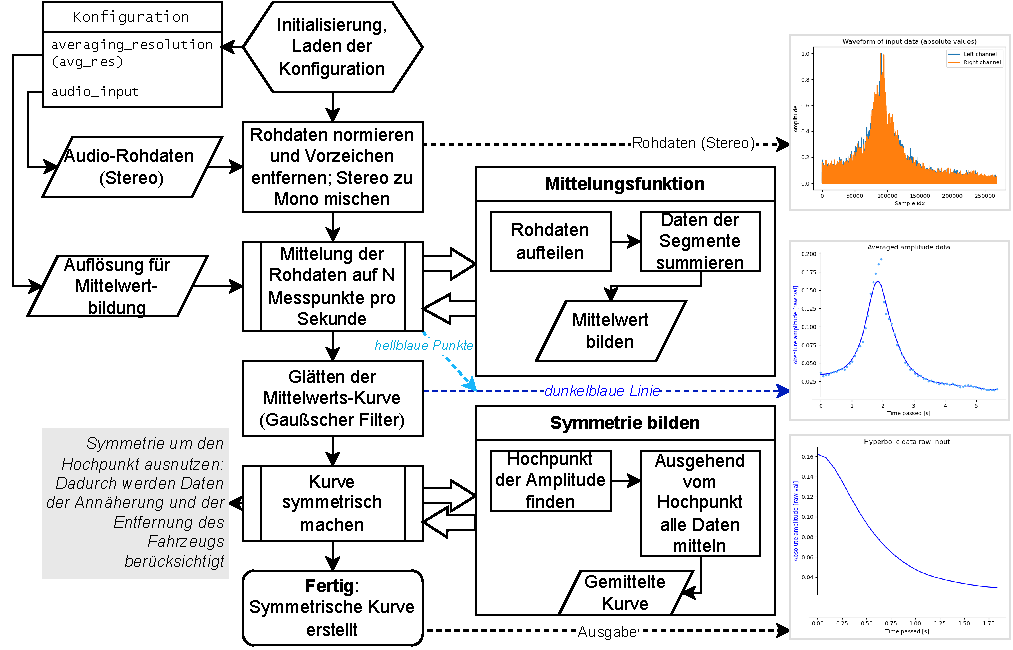
\includegraphics[width=\textwidth]{AmplitudeAnalyser.pdf}
    \caption{Flussdiagramm zur Verarbeitung der Rohdaten, \(N\) empirisch ermittelt}
    \label{fig:flow_amp_analyser}
\end{figure}

\begin{figure}[h!]
    \begin{subfigure}{.45\textwidth}
        \centering
        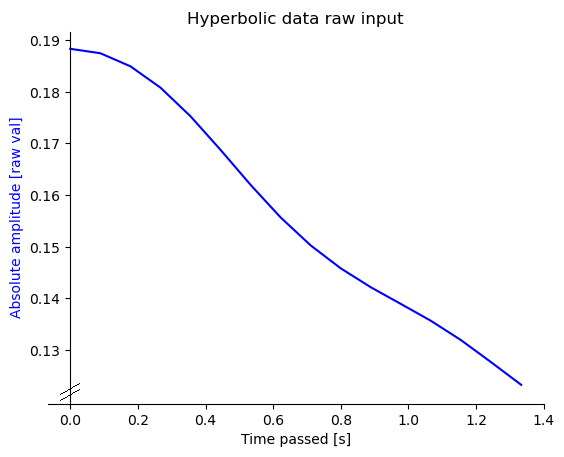
\includegraphics[width=.8\linewidth]{avg_symm_faulty}
        \caption{Gemittelte Rohdaten}
        \label{img:avg_symm_faulty}
    \end{subfigure}
    \begin{subfigure}{.45\linewidth}
        \centering
        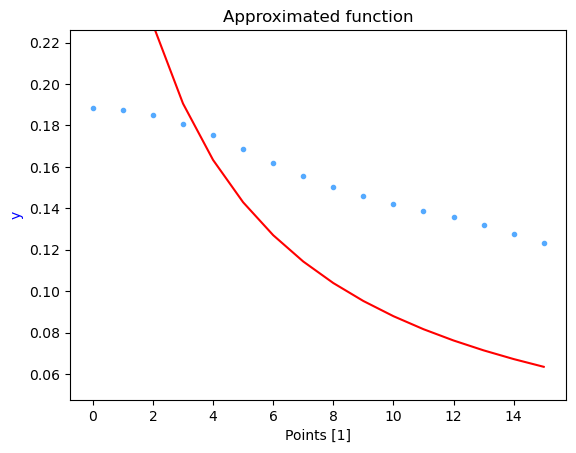
\includegraphics[width=.8\linewidth]{approx_function_faulty}
        \caption{Fehlerhafte angenäherte Funktion}
        \label{img:approx_function_faulty}
    \end{subfigure}
    \caption{Unbrauchbare Daten aufgrund von Mittelung}
    \label{img:faulty_averaging}
\end{figure}

Es stellte sich jedoch heraus, dass in einigen Aufnahmen die Mittelung von Annäherung und Entfernung sowie die Mittelung beider Stereokanäle ungeeignet ist (Beispiel siehe \autoref{img:faulty_averaging}). Der Mittelwert-Ansatz wurde deshalb verworfen, stattdessen wurden in der nächsten Version insgesamt vier Einzelkurven berechnet, pro Kanal eine für die Annäherung und eine für die Entfernung des Kfz. Der Einfachheit halber wird bei den folgenden Abbildungen nicht berücksichtigt, dass immer insgesamt vier Datenreihen verarbeitet werden.

Die Punkte der gemittelten Rohdaten werden im nächsten Schritt an die Kurvenannäherung weitergegeben.

\FloatBarrier
\subsubsection{Annäherung der Hyperbelfunktion}
Für die Vereinfachung der Geschwindigkeitsberechnung wird im nächsten Schritt auf die gemittelten Rohdaten eine Hyperbelfunktion angenähert, da sich der Schalldruck umgekehrt proportional zum Abstand von Messgerät und Schallquelle verhält, wie in \autoref{section:AnalyseAudiodatenPegel} bereits beschrieben. Ausschlaggebendes Merkmal einer Hyperbel \(f(x) = a * \frac{1}{x}\) ist deren Streckfaktor \(a\). Im konkreten Anwendungsfall existiert keine Verschiebung der Funktion entlang der x-Achse, da der Hochpunkt der Rohdaten an der Stelle \(x = 0\) liegt. Ebenso wird die Verschiebung entlang der y-Achse nicht berücksichtigt, da der hyperbelförmige Teil der Aufnahme einer nicht verschobenen Funktion entspricht.

Der Annäherungsalgorithmus funktioniert prinzipiell mit jeder beliebigen mathematischen Funktion und besteht aus zwei wesentlichen Teilen:
\begin{enumerate}
    \item Eine Gütefunktion bestimmt die Abweichung der approximierten Funktion zu den Messwerten.
    \item Über einen rekursiven Ansatz wird das Extremwertproblem gelöst, die Güte zu maximieren beziehungsweise die Abweichung zu minimieren.
\end{enumerate}

Die Gütefunktion gewichtet dabei Werte mit größerem $x$-Wert stärker, da die Rohdaten aufgrund der \emph{nicht} unendlich groß werdenden Amplituden nahe \(0\) keiner Hyperbel mehr entsprechen. Das ist gleichzeitig eine Grenze des Annäherungs-Ansatzes.

\autoref{fig:flow_curve_fitter} beschreibt vereinfacht den rekursiven Ablauf der Annäherung des Hyperbel-Streckfaktors.

\begin{figure}[h]
    \centering
    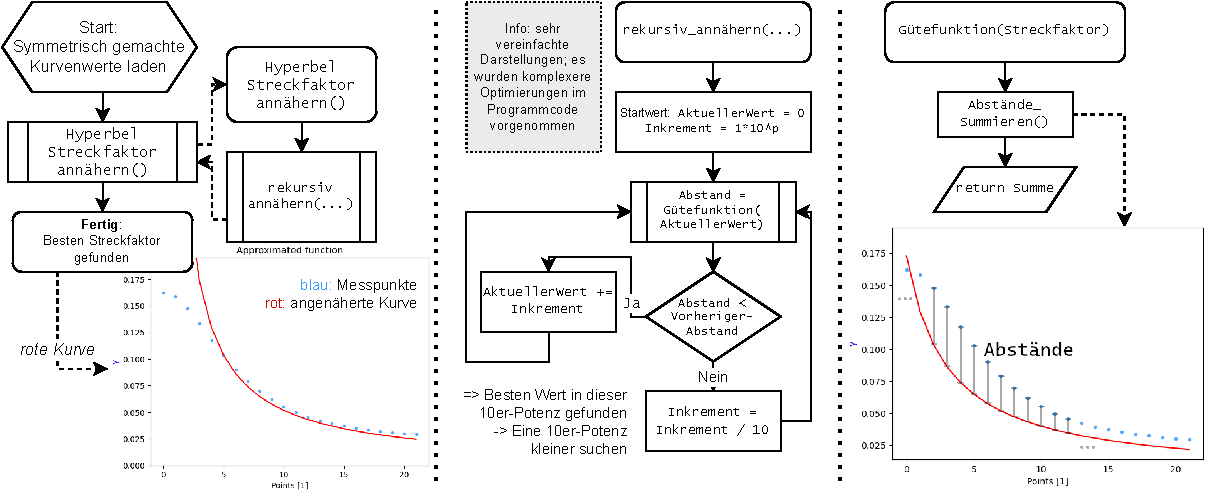
\includegraphics[width=\textwidth]{CurveFitter.pdf}
    \caption{Flussdiagramm zur Annäherung der Hyperbel}
    \label{fig:flow_curve_fitter}
\end{figure}

In \autoref{fig:ex_hyperbel_approx} wurde anhand eines trivialen Beispiels der Ablauf der Annäherung dargestellt. Das Beispiel ist trivial, da „Abstand“ hier den Abstand der aktuellen Annäherung („Versuch“) auf dem Zahlenstrahl darstellt. Bei der Annäherung der Hyperbel wird der „Abstand“ jedoch von einer Gütefunktion berechnet, wie in \autoref{fig:flow_curve_fitter} (rechts) dargestellt.

\begin{figure}[h]
    \centering
    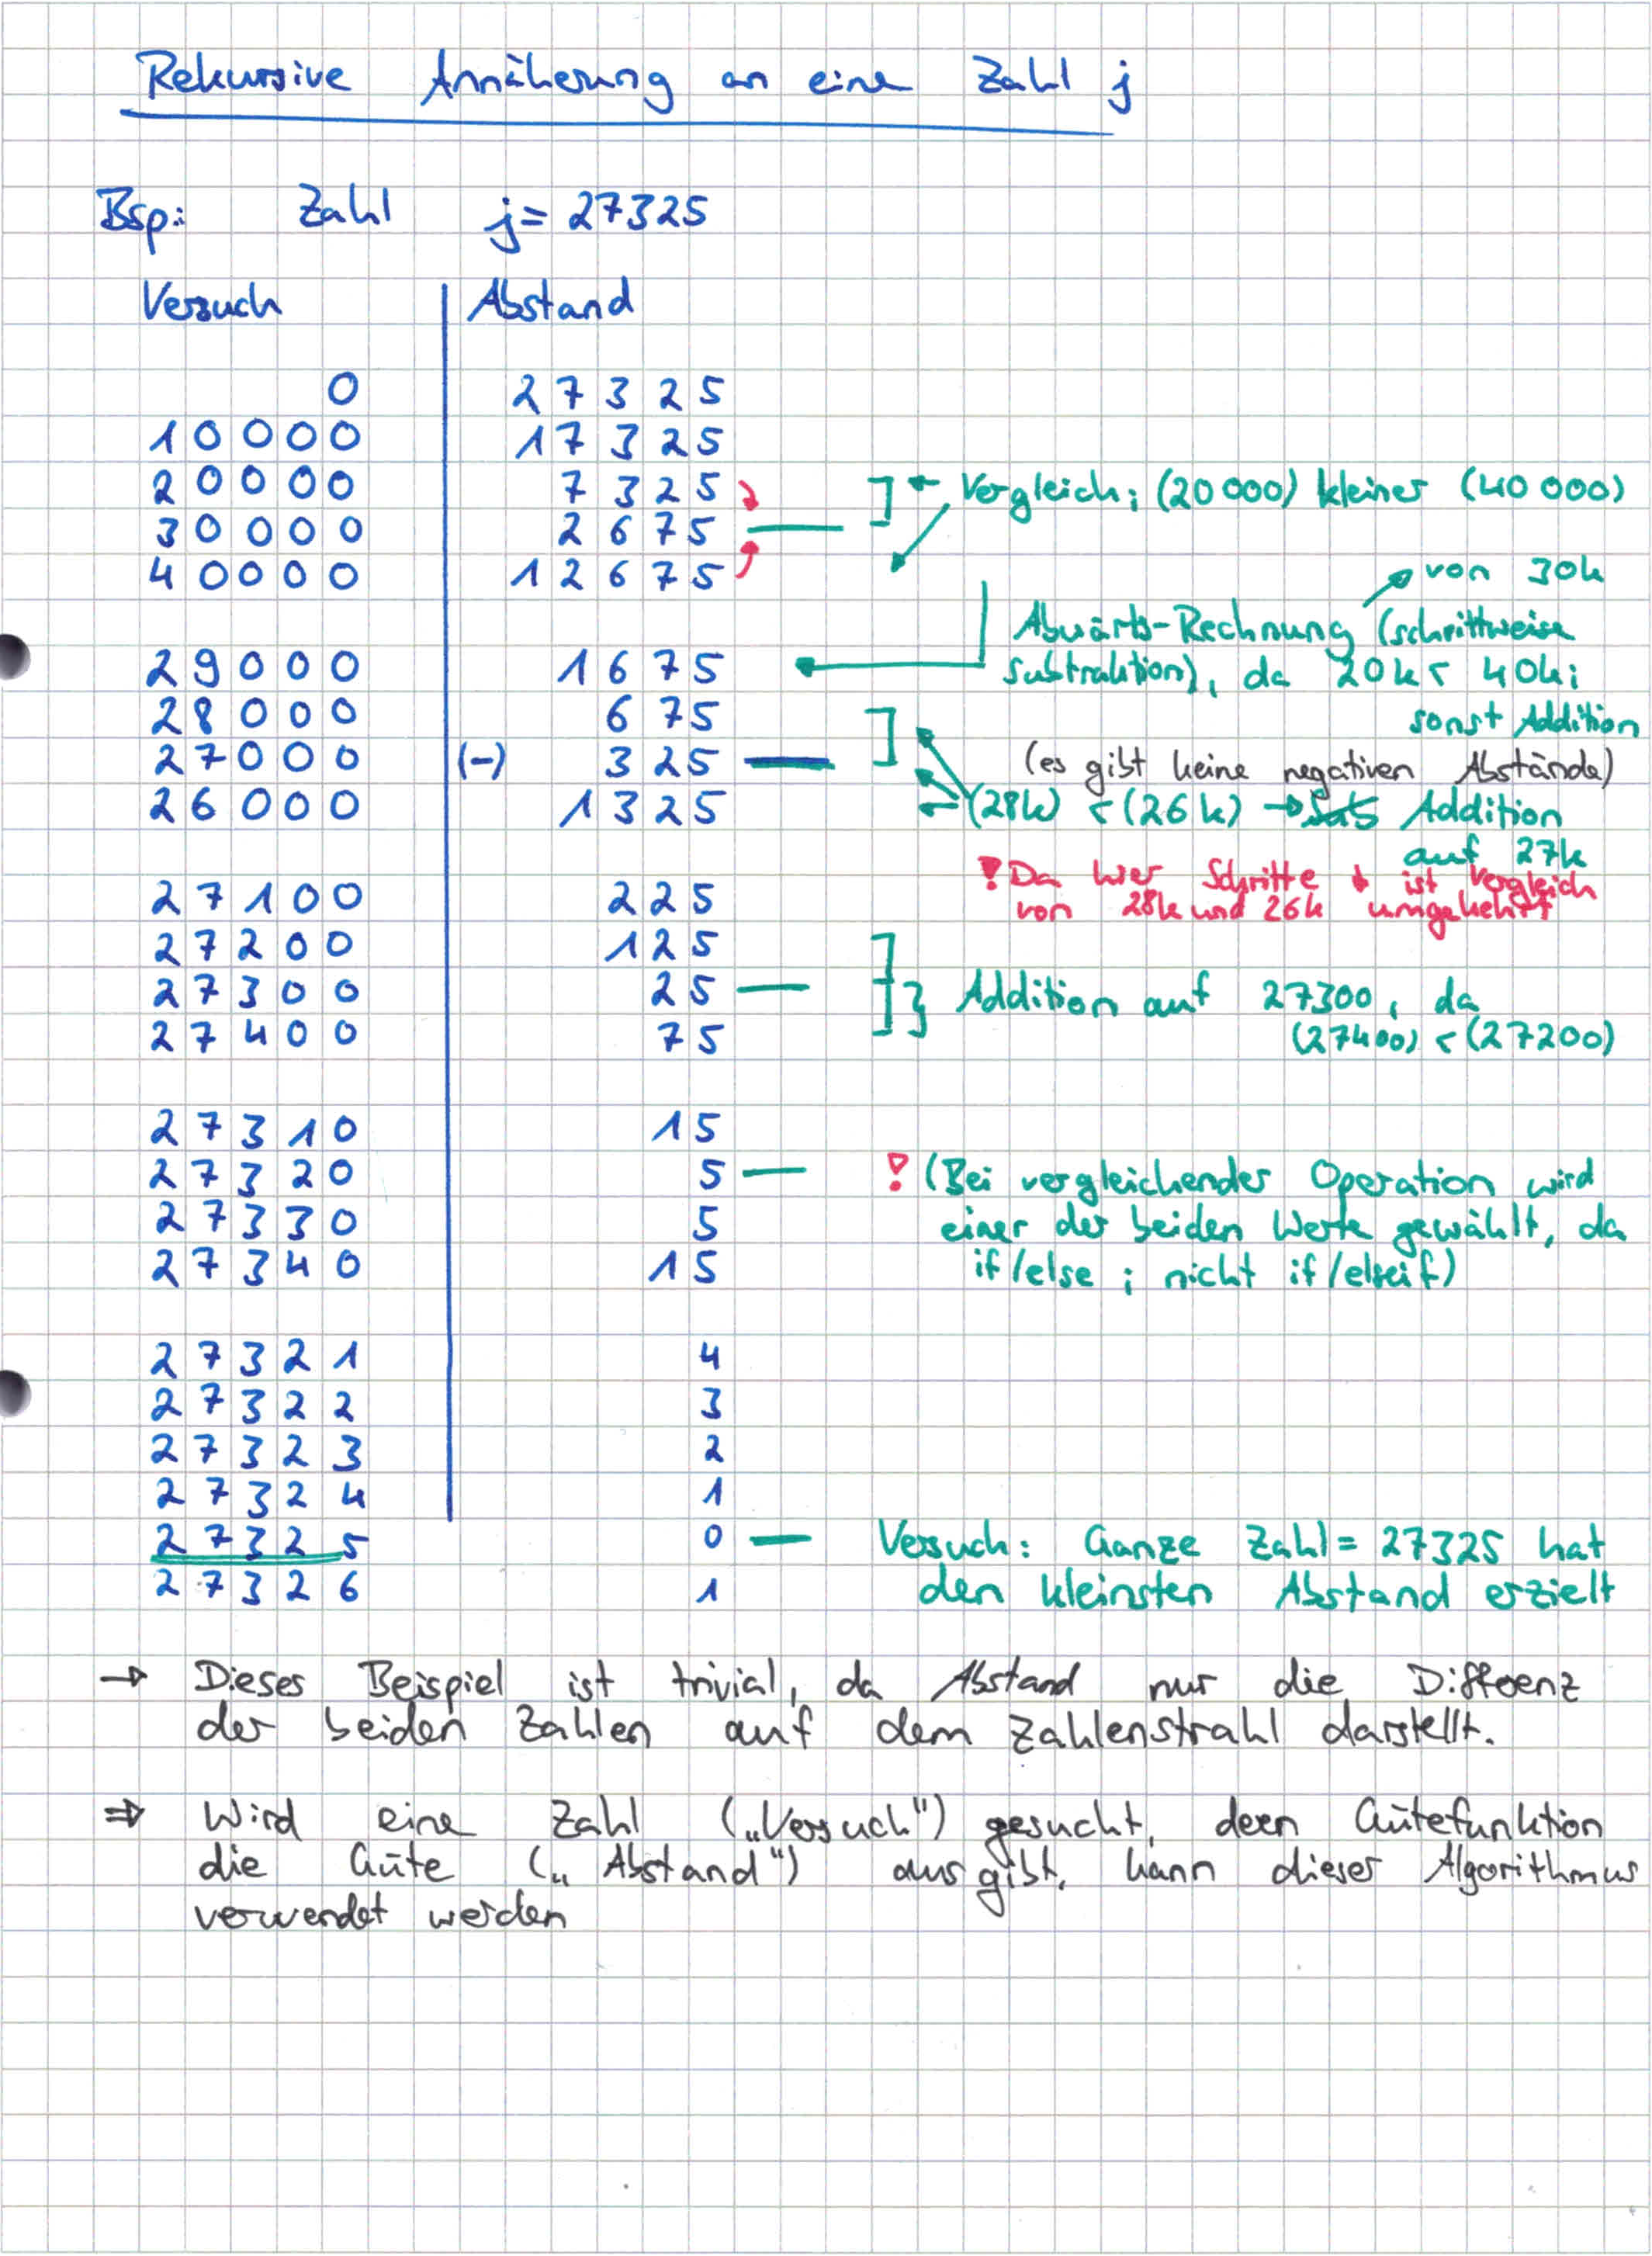
\includegraphics[width=\textwidth]{HyperbelApproxBsp}
    \caption{Triviales Beispiel zur Annäherung der Hyperbel}
    \label{fig:ex_hyperbel_approx}
\end{figure}

\FloatBarrier
\subsubsection{Geschwindigkeitsberechnung}
Im dritten Schritt wird zunächst die Amplitudenfunktion in eine Funktion des effektiven Schalldruckpegels (RMS) über Zeit umgerechnet. Diese Umrechnung geschieht in zwei Schritten: Zuerst wird der Effektivwert (Root Mean Square, RMS) der Amplitude berechnet \cite{SiemensRMS}, um nicht in Grenzfälle, wie \(a = 0 \longrightarrow L(0) = -\infty\), zu geraten. Anschließend wird die Amplitude in einen Pegel umgerechnet, da bei Pegeln die „\(6 dB\)-Abstandsregel“ angewendet werden kann.
\begin{equation}
    \begin{split}
        L_{amplitude}(a) = 20 * \log(a) \\
        L_{RMS}(a) = L_{amplitude}\left(\sqrt{\frac{a^2}{2}}\right)
    \end{split}
    \label{equation:LRMS}
\end{equation}

Für eine Geschwindigkeitsberechnung bei näherungsweise gleichförmiger Bewegung des vorbeifahrenden Fahrzeugs kann die Formel \(v = \frac{\Delta s}{\Delta t}\) verwendet werden. Für die Berechnung des Wegunterschieds wird zweimal auf \autoref{equation:RadiusAusSchallpegel} zurückgegriffen, um die Abstände von Mikrofon und Fahrzeug an zwei beliebigen Punkten der angenäherten Hyperbel-Kurve zu berechnen. Die Wahl der Punkte spielt hierbei keine Rolle, da die Pegelfunktion einer reinen Logarithmusfunktion entspricht, weil diese aus der angenäherten Hyperbel und nicht aus Rohdaten berechnet wurde. Der Einfachheit halber und um Rundungsfehler zu minimieren, wurden die Punkte bei \(x_{2} = \frac{1}{3} * len, \quad x_{3} = \frac{2}{3} * len\) für die Berechnung gewählt sowie der Referenzwert \(x_{1} = d_{a}\) (\(d_{a}\): Abstand vom Mikrofon zur Straße) mit \(L_{1} = 0 dB\). \(len\) ist hierbei die Länge der Liste der Messpunkte.

Mithilfe von \autoref{equation:RadiusAusSchallpegel}:
\begin{equation*}
    \begin{split}
        r_{2} = r_{1} * 10^{\left(\frac{\abs{L_{1} - L_{2}}}{20}\right)} \\
        d_{2} = \sqrt{r_{2}^2 - d_{a}^2}
    \end{split}
\end{equation*}
kann für \(r_{1} = d_{a}\) und für \(L_{1} = 0 dB\) eingesetzt werden. \(L_{2}\) wird daraufhin aus der Funktion des effektiven Schalldruckpegels (\autoref{equation:LRMS}) an den Stellen \(x_{2}\) und \(x_{3}\) berechnet und eingesetzt. Die beiden berechneten Abstände \(d_{2}\) und \(d_{3}\) werden verwendet, um die Geschwindigkeit zu berechnen:
\[
    v_{2,3} = \frac{d_{3} - d_{2}}{\Delta t_{2,3}}
\]

Da \(d\) üblicherweise in Metern und \(t\) in Sekunden angegeben wird, muss für eine Geschwindigkeit in Kilometern pro Stunde \(v_{2,3}\) noch mit \(3,6\) multipliziert werden. Somit wurde die Geschwindigkeit \(v\) eines vorbeifahrenden Fahrzeugs anhand der Lautstärkeänderung berechnet.